% title: Feedback through two executed while-loop steps
% description: Two body calls take the initial state s0 to s1 and then s2. The backward pass starts with feedback for s2 and applies the body pullback at the saved states s1 and s0, in that order. The result is feedback for the initial state. Solid arrows carry states; dashed arrows carry feedback.
\documentclass[tikz,border=5pt]{standalone}
\usetikzlibrary{arrows.meta,calc,shapes.geometric}
\definecolor{numeric}{HTML}{4477AA}
\definecolor{textual}{HTML}{AA4499}

\tikzset{
    box/.style={draw, line width=0.8pt, minimum height=0.8cm,
                minimum width=1.8cm, inner sep=6pt, align=center},
    ir/.style={box},
    flow/.style={-{Stealth[length=5pt]}, line width=0.9pt},
    feedback/.style={flow, dashed},
    note/.style={font=\small, align=center},
    choice/.style={diamond, draw, line width=0.8pt,
                   aspect=2, inner sep=2pt, align=center},
}

\newcommand{\irframe}[2]{
    \draw[line width=0.8pt] #1 rectangle #2;
}

\newcommand{\transformarrow}[4][above]{
    \draw[flow] (#2) -- node[#1=6pt,note] {#4} (#3);
}

\begin{document}
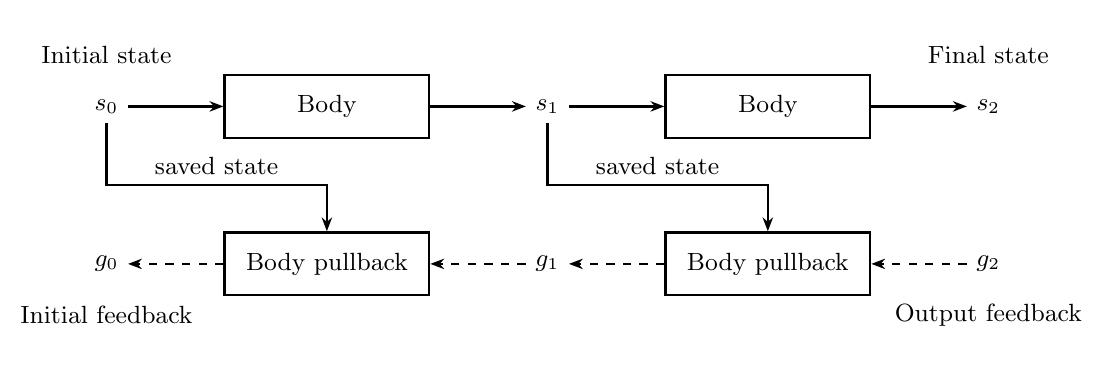
\begin{tikzpicture}[font=\small]
    \path[use as bounding box] (-6.6,-2.05) rectangle (6.6,2.0);

    \node (initial) at (-5.6,1.0) {$s_0$};
    \node[box, minimum width=2.6cm] (stepone) at (-2.8,1.0) {Body};
    \node (middle) at (0,1.0) {$s_1$};
    \node[box, minimum width=2.6cm] (steptwo) at (2.8,1.0) {Body};
    \node (final) at (5.6,1.0) {$s_2$};
    \node[note] at (-5.6,1.65) {Initial state};
    \node[note] at (5.6,1.65) {Final state};

    \draw[flow] (initial) -- (stepone);
    \draw[flow] (stepone) -- (middle);
    \draw[flow] (middle) -- (steptwo);
    \draw[flow] (steptwo) -- (final);

    \node (initialfeedback) at (-5.6,-1.0) {$g_0$};
    \node[box, minimum width=2.6cm] (pullone) at (-2.8,-1.0) {Body pullback};
    \node (middlefeedback) at (0,-1.0) {$g_1$};
    \node[box, minimum width=2.6cm] (pulltwo) at (2.8,-1.0) {Body pullback};
    \node (outputfeedback) at (5.6,-1.0) {$g_2$};
    \node[note] at (-5.6,-1.65) {Initial feedback};
    \node[note] at (5.6,-1.65) {Output feedback};

    \draw[feedback] (outputfeedback) -- (pulltwo);
    \draw[feedback] (pulltwo) -- (middlefeedback);
    \draw[feedback] (middlefeedback) -- (pullone);
    \draw[feedback] (pullone) -- (initialfeedback);

    \draw[flow] (initial.south) -- (-5.6,0)
        -- node[above,note] {saved state} (-2.8,0) -- (pullone.north);
    \draw[flow] (middle.south) -- (0,0)
        -- node[above,note] {saved state} (2.8,0) -- (pulltwo.north);
\end{tikzpicture}
\end{document}
